\chapter{Chordal Graphs}
\section{What makes a graph Chordal?}
A \textbf{Chord} is an edge in a graph that connects two non-adjacent vertices that are apart of the same cycle. (note: cycles of size three cannot have chords in undirected graphs)\\
A graph G is \textbf{Chordal} if every cycle above size greater than four has at least one chord.\\

\section{What Do Chordal Graphs Look Like?}
What do \textbf{Chords} look like? The following two graphs are examples of chordal graphs, one with 5 vertices, and another with 8 vertices. The chordal lines are visible in green.
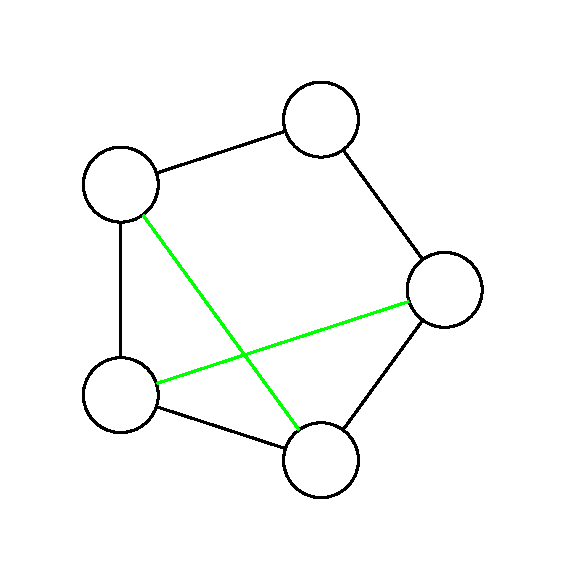
\includegraphics[width=0.5\textwidth]{./ChapterChordal/chordalGraph.pdf}
\includegraphics[width=0.5\textwidth]{./ChapterChordal/chordalGraph2.pdf}

However, as described earlier, not all graphs with cycles are \textbf{Chordal}. For example, while this graph does have greater than four vertices, the cycle condition is not met.
\includegraphics[width=0.5\textwidth]{./ChapterChordal/nonchordalGraph.pdf}


\section{How are they Used?}
The cyclical and proximity-based nature of chordal graphs allows them to be used in a variety of ways. They are often used to organize
tasks efficiently, or to highlight relations inside data clusters. A common place chordal graphs are seen is in the implementation of algorithms to build
massive graphs representing the phylogenetic trees of evolutionary species. This has been a topic of study in computational biology; generated chordal
graphs allow scientists to create a constructive heuristic based on the degree of relation between species on the general evolutionary tree. ~\cite{kennedy_2005}
Researchers can easily add constraints to chordal graphs, making them a good choice for sorting complex data sets with custom parameters.\par
Another modern application of chordal graphs is in the area of computer optimization. Like most graphs, chordals are also applied to the study of
register allocation. Variables stored in registers can be tracked better and allocated in relation to other variables using a chordal graph alongside
static single assignment to lump declarations together, allowing for a more optimized system of register allocation. ~\cite{hack_2007} Interestingly, chordal graphs
can be colored to produce similar efficiency-based algorithms. There have been studies into how these two components of graph theory can work together to
form powerful and competent register allocation patterns. \cite{pereira_palsberg}\\

\section{What problems do chordal graphs help with?}



\url{http://digbib.ubka.uni-karlsruhe.de/volltexte/documents/6532}\\
\url{http://webdocs.cs.ualberta.ca/~hayward/theses/sean.pdf}\\
\url{http://web.cs.ucla.edu/~palsberg/paper/aplas05.pdf}

\bibliographystyle{plain}
\bibliography{ChapterChordal/bibliography.bib}
